%Appendices
\begin{appendices}
	\renewcommand{\thechapter}{\Roman{chapter}}	

\chapter{Simulation process flow schematics}\label{Schematics}
\clearpage
	
	\begin{figure}[h!]
		\centering
		\fbox{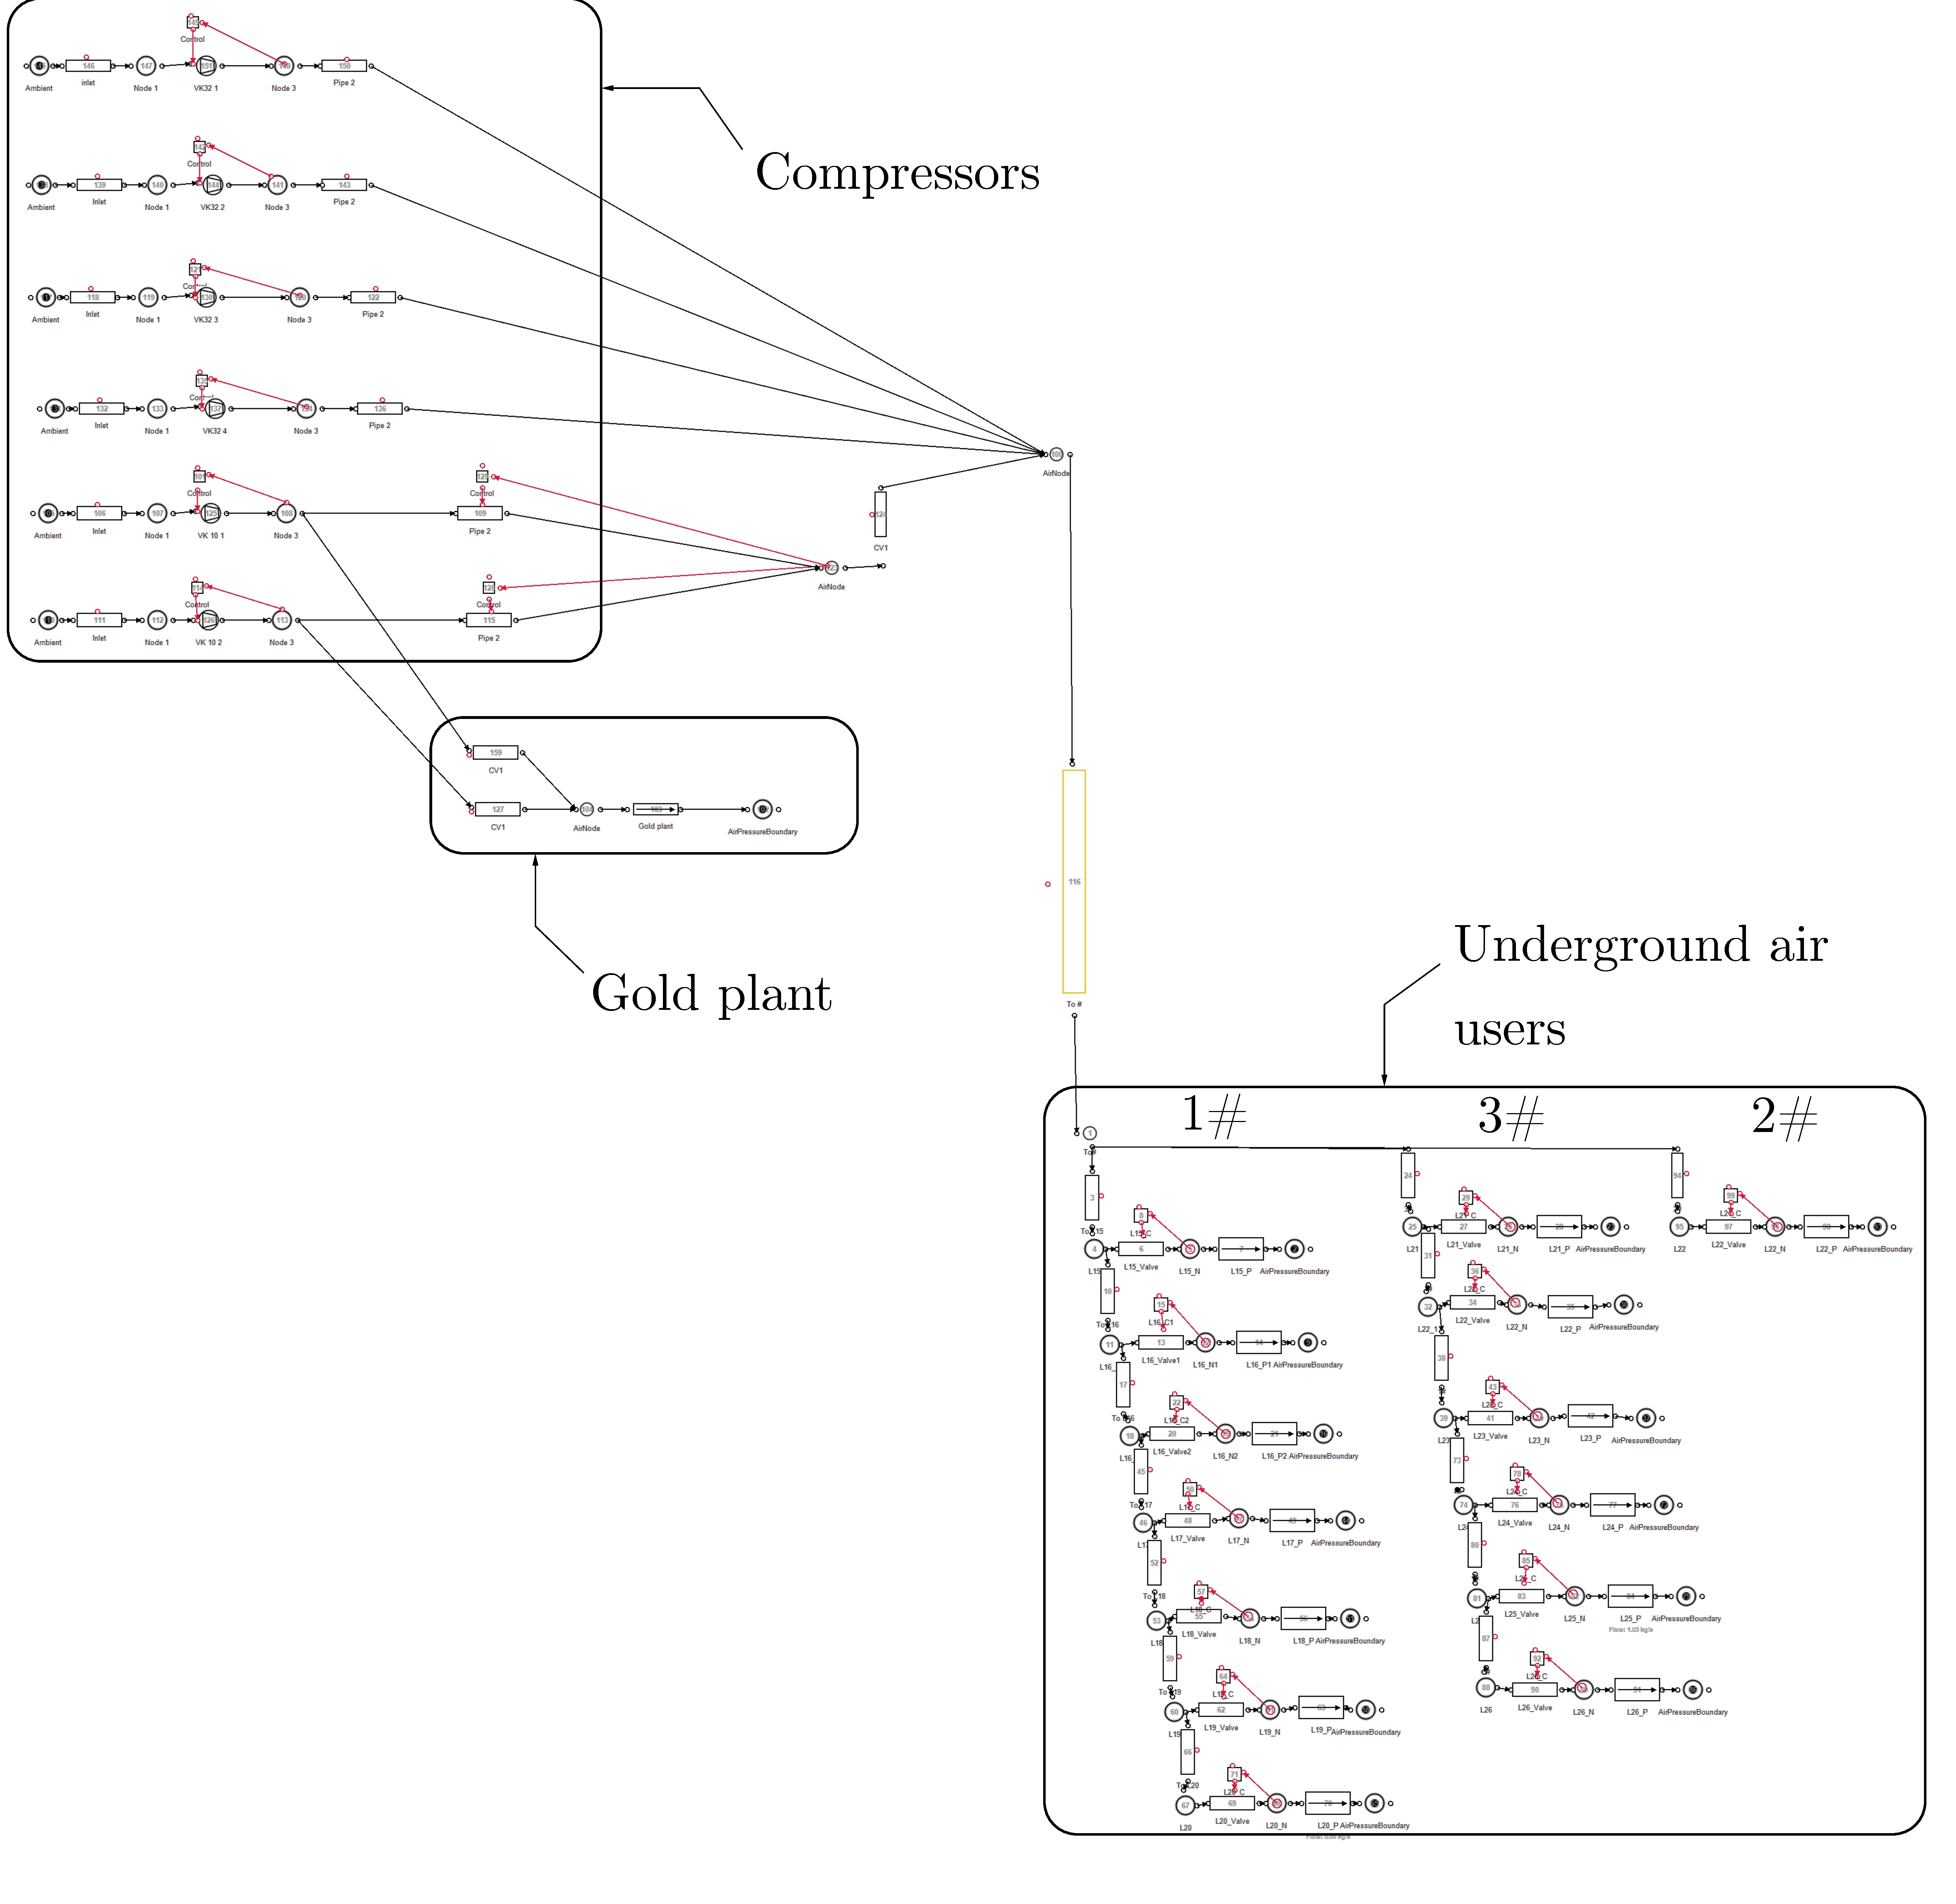
\includegraphics[width=\textwidth]{Images/A/Beet/BeetSim.pdf}}
		\caption{Mine A: Simulation process flow schematic}
		\label{fig: BEET Baseline model}
	\end{figure}
	\clearpage
	
	%%%% KUS Baseline %%%%
	\begin{figure}[h!]
		\centering
		\fbox{\includegraphics[trim =0cm 0 0cm 0cm,width=\textwidth]{Images/A/Kus/Baseline.pdf}}
		\caption{Mine B:  Baseline process flow schematic}
		\label{fig: KUS Baseline model}
	\end{figure}
	\clearpage
	\begin{figure}[h!]
		\centering
		\fbox{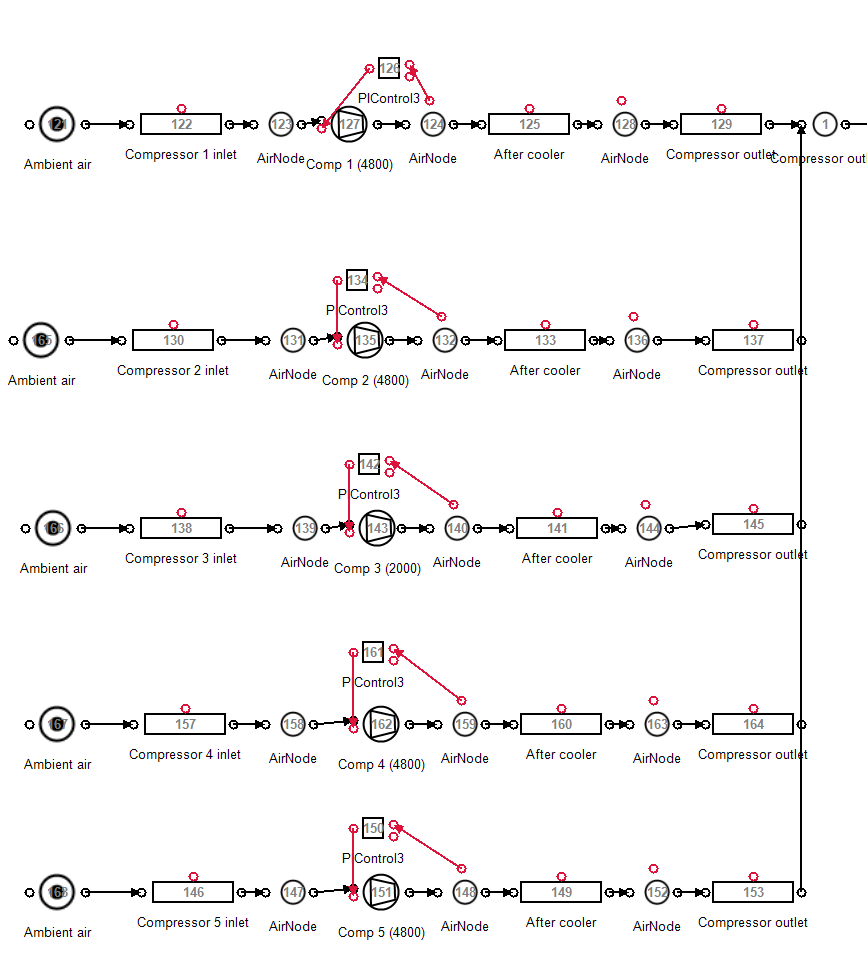
\includegraphics[trim =0cm 0 0cm 0cm,width=0.8\textwidth]{Images/A/Kus/compressors}}
		\caption{Mine B:  Compressors}
		\label{fig: KUS compressors model}
	\end{figure}
\hspace{1cm}
\begin{figure}[h!]
	\centering
	\fbox{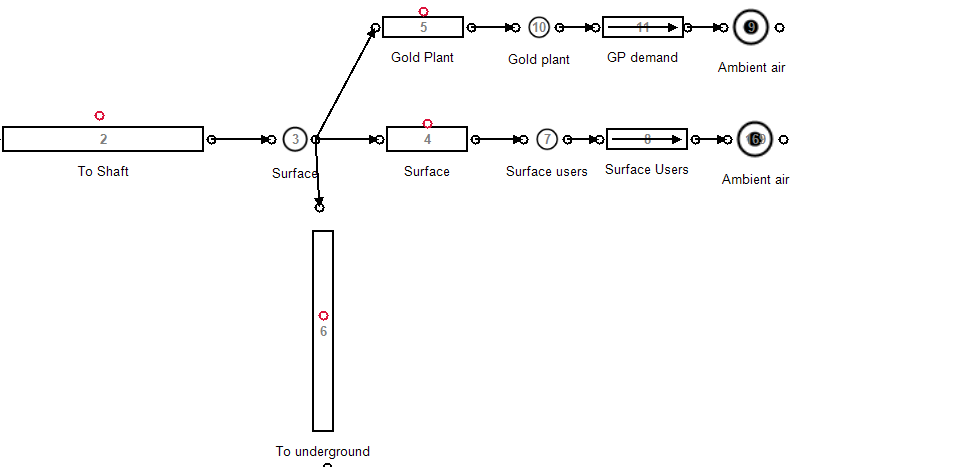
\includegraphics[trim =0cm 0 0cm 0cm,width=0.8\textwidth]{Images/A/Kus/surface}}
	\caption{Mine B: surface compressed air users}
	\label{fig: KUS surface model}
\end{figure}
\clearpage
\begin{figure}[h!]
	\centering
	\fbox{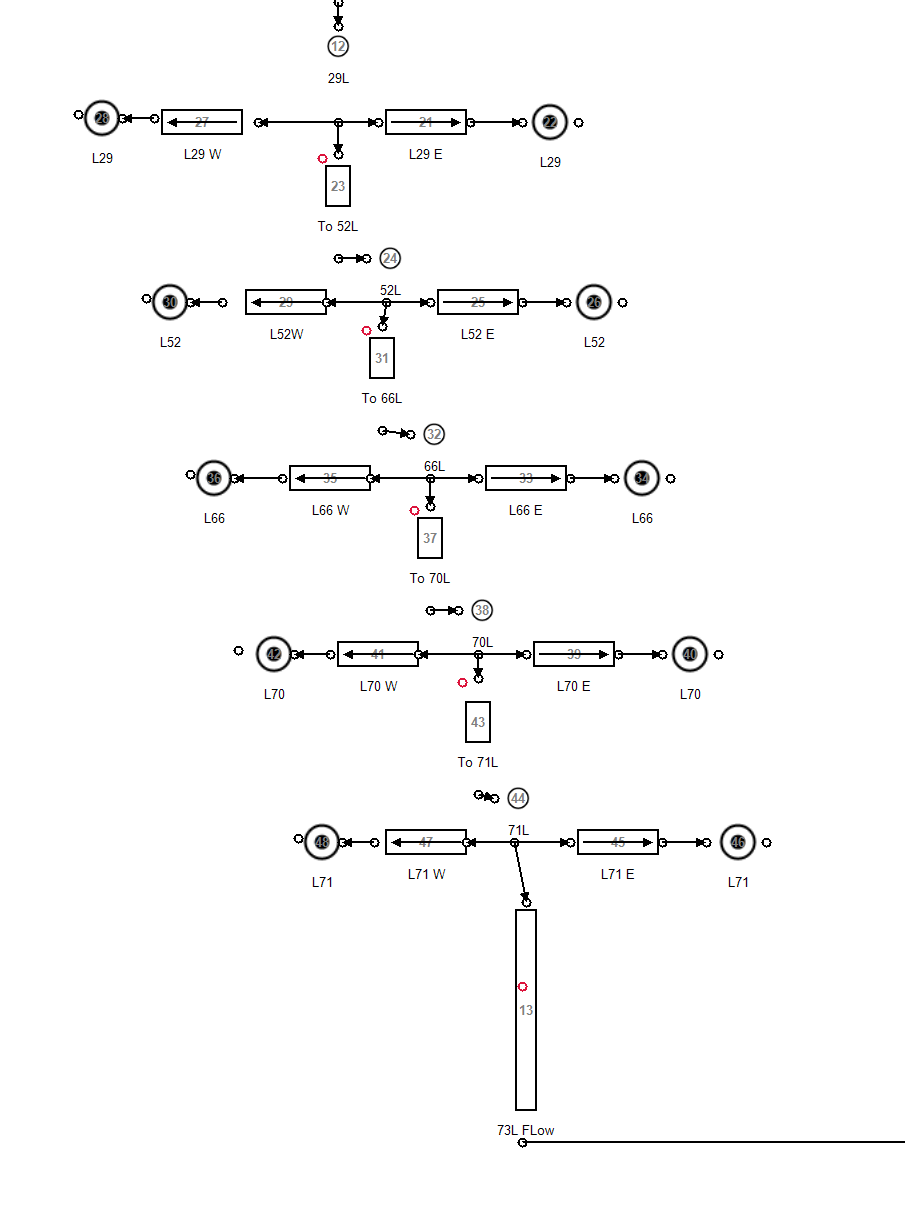
\includegraphics[trim =0cm 0 0cm 0cm,width=0.8\textwidth]{Images/A/Kus/main}}
	\caption{Mine B: Main shaft compressed air users}
	\label{fig: KUS main model}
\end{figure}
\clearpage
\begin{figure}[h!]
	\centering
	\fbox{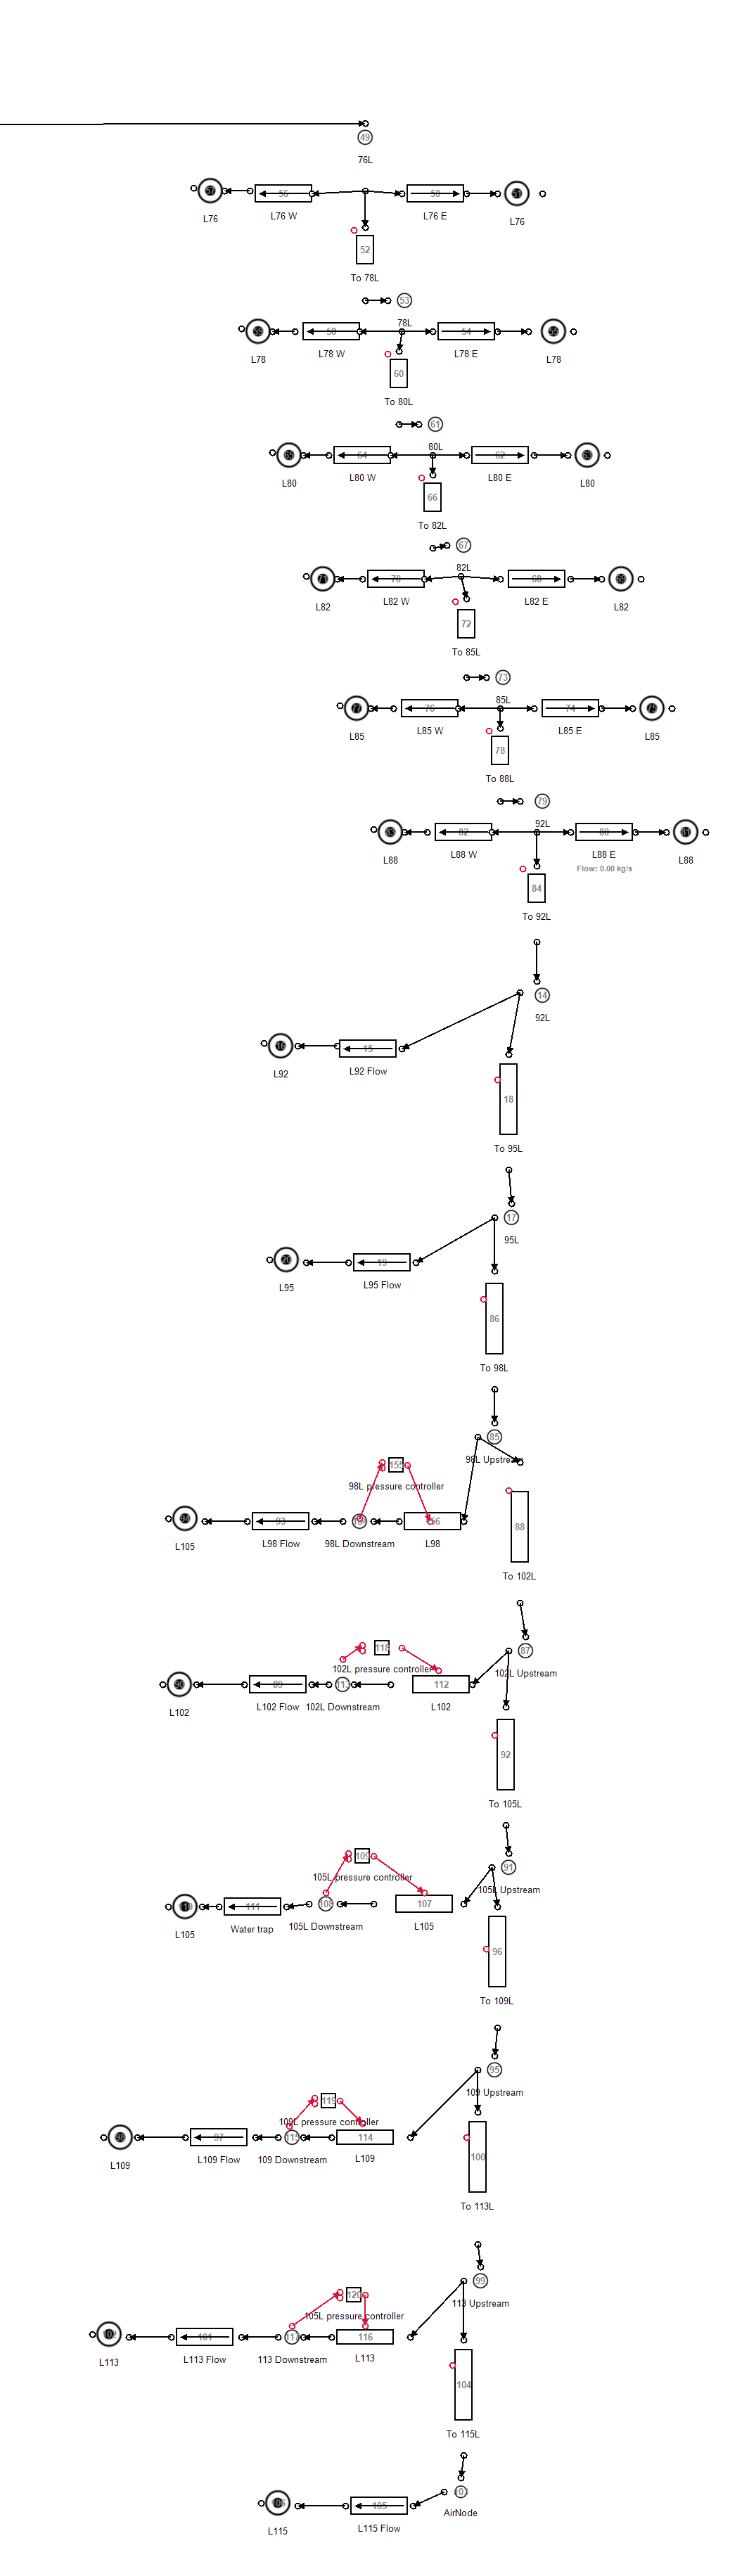
\includegraphics[trim =0cm 0 0cm 0cm,width=0.42\textwidth]{Images/A/Kus/sub}}
	\caption{Mine B: Sub-shaft compressed air users}
	\label{fig: KUS sub model}
\end{figure}

%%%%%% Refuge bays
	\begin{figure}[h]
		\centering
		\fbox{\includegraphics[trim =-35cm 0 -35cm 0cm,width=\textwidth]{Images/A/RefBaySim2}}
		\caption{Mine B: Simulation process flow diagrams for the refuge bay scenario.}
		\label{fig: Refuge bay layout}
	\end{figure}	

	\begin{figure}[h]
		\centering
		\fbox{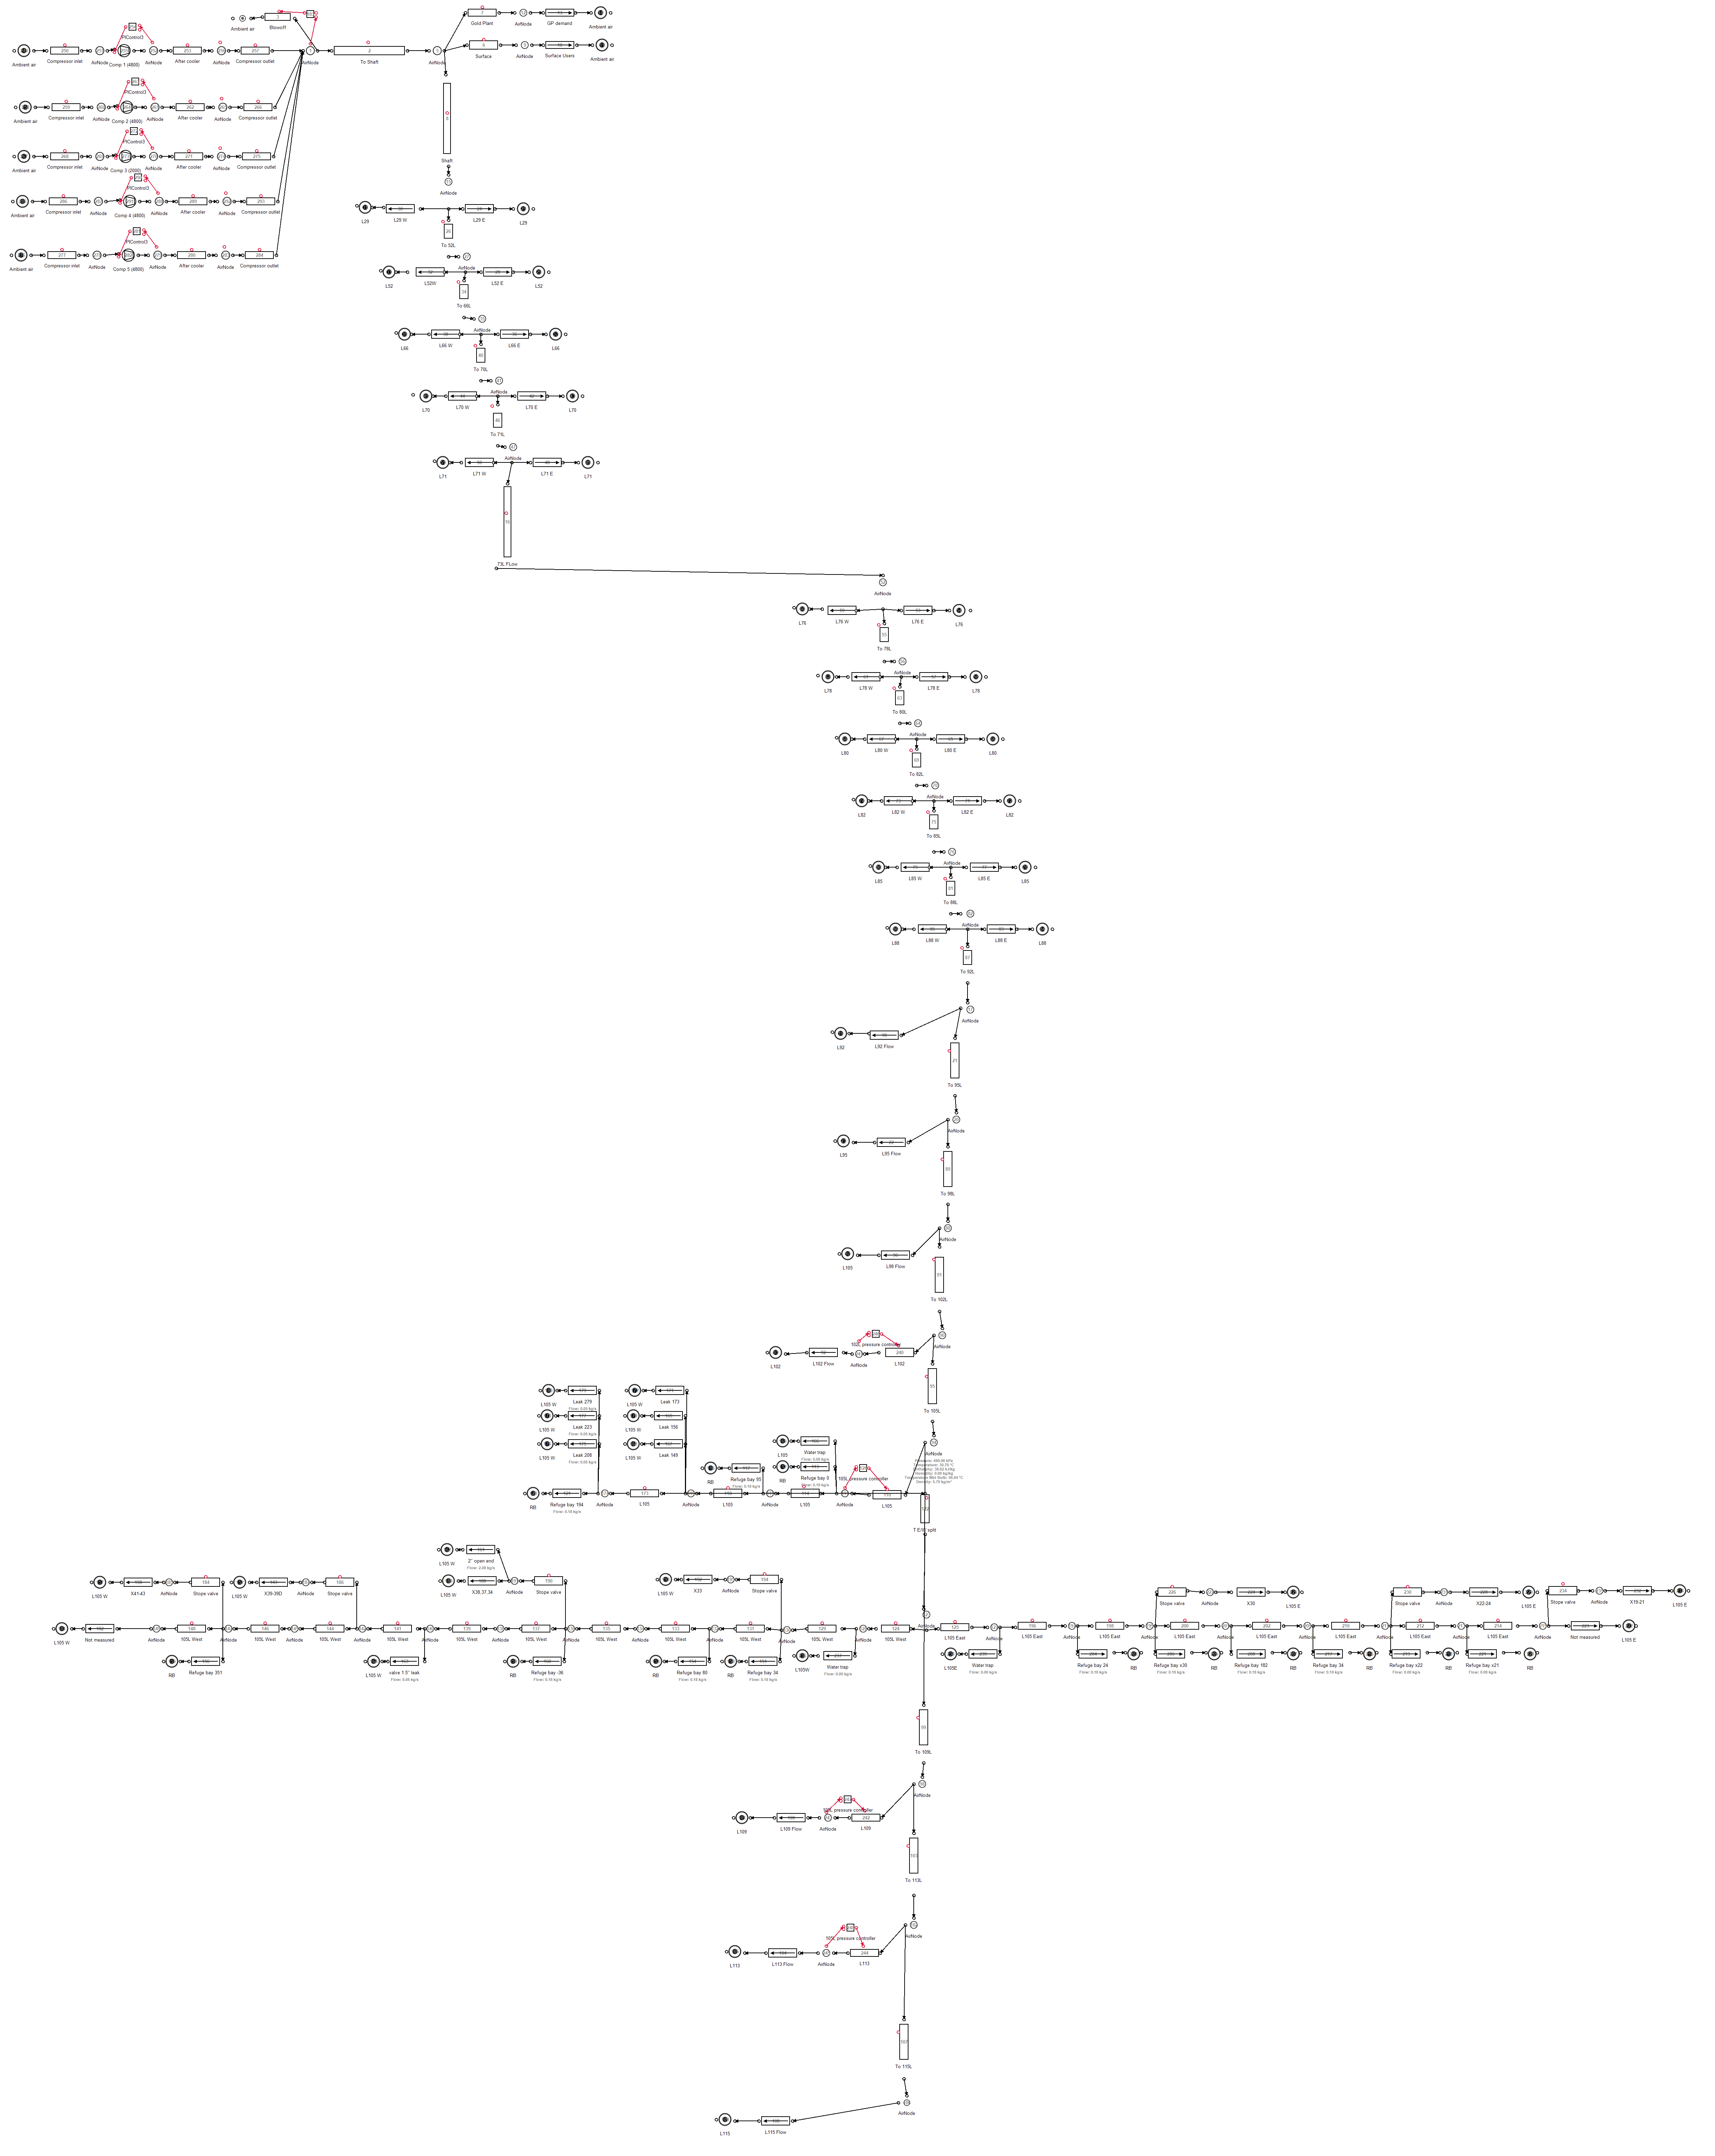
\includegraphics[trim = 0.8cm 5.8cm  0.8cm 5.8cm ,clip,width=\textwidth]{Images/A/StopeSim.png}}
		\caption{Mine B: Simulation process flow diagram for the station isolation stope control.}
		\label{fig: Stope layout}
	\end{figure}
\chapter{Model components verification tables}
\newpage
\begin{table}[h!]
	\centering
	\begin{tabular}{lccr}
		\hline 
		Component & Actual Ave. & Simulated  Ave. & Accuracy \\ \hhline{====} 
		\\
		\multicolumn{4}{c}{Power ($ kW $)}
		\\
		VK-32 1 & $  0  $ & $  0  $ & $ 100   $\% \\
		VK-32 2 & $ 460 $ & $ 477 $ & $ 96.35 $\% \\
		VK-32 3 & $ 142 $ & $ 117 $ & $ 82.31 $\% \\
		VK-32 4 & $ 428 $ & $ 408 $ & $ 95.45 $\% \\
		VK-32 5 & $ 1813$ & $ 1903$ & $ 95.03 $\% \\
		VK-32 6 & $ 732 $ & $ 725 $ & $ 99.01 $\% \\
		VK-10 1 & $ 744 $ & $ 745 $ & $ 90.02 $\% \\
		VK-10 2 & $ 687 $ & $ 635 $ & $ 92.24 $\% \\
		System  & $ 4940$ & $4911 $ & $ 97.34 $\% \\
		\\
		\multicolumn{4}{c}{Flow ($ kg/s $)}
		\\
		1\# 15L  & $ 1.45 $ & $ 1.42 $ & $ 97.87 $\% \\
		1\# 16L  & $ 2.15 $ & $ 2.18 $ & $ 98.48 $\% \\
		1\# 17L  & $ 0.34 $ & $ 0.35 $ & $ 97.30 $\% \\
		1\# 18L  & $ 0.38 $ & $ 0.39 $ & $ 97.39 $\% \\
		1\# 19L  & $ 0.31 $ & $ 0.31 $ & $ 98.77 $\% \\
		1\# 20L  & $ 0.12 $ & $ 0.13 $ & $ 92.65 $\% \\
		2\# 23L  & $ 1.31 $ & $ 1.35 $ & $ 96.69 $\% \\
		3\# 21L  & $ 0.67 $ & $ 0.66 $ & $ 98.68 $\% \\
		3\# 22L  & $ 0.74 $ & $ 0.67 $ & $ 89.54 $\% \\
		3\# 23L  & $ 0.04 $ & $ 0.04 $ & $ 98.72 $\% \\
		3\# 24L  & $ 0.11 $ & $ 0.11 $ & $ 98.76 $\% \\
		3\# 25L  & $ 0.33 $ & $ 0.33 $ & $ 99.95 $\% \\
		3\# 26L  & $ 0.45 $ & $ 0.47 $ & $ 95.07 $\% \\
		Gold Plant & $ 2.59 $ & $ 2.48 $ & $ 95.72 $\% \\
		Total  	 & $ 9.32$  & $9.51 $  & $ 97.01 $\% \\
		\hline 
	\end{tabular}
		\caption{Case study A: Model verification}
		\label{Table: A verification}
	\end{table}
\begin{table}[h!]
		\centering
		\begin{tabular}{lccr}
			\hline 
			Component & Actual Ave. & Simulated  Ave. & Accuracy \\ \hhline{====} 
			\\
		\multicolumn{4}{c}{Pressure ($ kPa $)}
		\\
		1\# 15L  & $ 394 $ & $ 384 $ & $ 98.55 $\% \\
		1\# 16L  & $ 421 $ & $ 419 $ & $ 99.61 $\% \\
		1\# 17L  & $ 345 $ & $ 344 $ & $ 99.81 $\% \\
		1\# 18L  & $ 336 $ & $ 336 $ & $ 99.99 $\% \\
		1\# 19L  & $ 311 $ & $ 309 $ & $ 99.53 $\% \\
		1\# 20L  & $ 368 $ & $ 368 $ & $ 99.90 $\% \\
		2\# 23L  & $ 365 $ & $ 327 $ & $ 91.25 $\% \\
		3\# 21L  & $ 303 $ & $ 302 $ & $ 99.92 $\% \\
		3\# 22L  & $ 332 $ & $ 301 $ & $ 95.42 $\% \\
		3\# 23L  & $ 332 $ & $ 332 $ & $ 99.98 $\% \\
		3\# 24L  & $ 413 $ & $ 409 $ & $ 99.10 $\% \\
		3\# 25L  & $ 413 $ & $ 409 $ & $ 99.01 $\% \\
		3\# 26L  & $ 515 $ & $ 509 $ & $ 98.99 $\% \\
		Surface & $ 502 $ & $ 501 $ & $ 99.95 $\% \\
		\hline 
	\end{tabular}
\caption{Case study A: Model verification continued}
\label{Table: A verification2}
\end{table}

\newpage
\begin{table}[h!]
	\centering
	\begin{tabular}{lccr}
		\hline 
		Component & Actual Ave. & Simulated  Ave. & Accuracy \\ \hhline{====} 
		\\
		\multicolumn{4}{c}{Power ($ kW $)}
		\\
		Compressor 1 & $ 3406 $ & $ 3669 $ & $ 92.37 $\% \\
		Compressor 2 & $ 3911 $ & $ 3668 $ & $ 93.92 $\% \\
		Compressor 3 & $ 1440 $ & $ 1453 $ & $ 99.05 $\% \\
		Compressor 4 & $  0   $ & $  0   $ & $ 100   $\% \\
		Compressor 5 & $ 3299 $ & $ 3274 $ & $ 99.22 $\% \\
		System       & $12057 $ & $12103 $ & $ 98.73 $\% \\
		\\
		\multicolumn{4}{c}{Flow ($ kg/s $)}
		\\
		
		95L  & $ 1.51 $ & $ 1.42 $ & $ 93.95 $\% \\
		98L  & $ 3.75 $ & $ 3.53 $ & $ 93.99 $\% \\
		102L  & $ 2.97 $ & $ 2.79 $ & $ 98.72 $\% \\
		105L  & $ 5.65 $ & $ 5.71 $ & $ 98.84 $\% \\
		109L  & $ 3.57 $ & $ 3.37 $ & $ 94.27 $\% \\
		113L  & $ 5.09 $ & $ 4.84 $ & $ 95.05 $\% \\
		Gold Plant & $ 1.41 $ & $ 1.35 $ & $ 95.14 $\% \\
		Sub-shaft total & $ 34.12 $ & $ 34.76 $ & $ 98.09 $\% \\
		Total & $ 41.65$  & $41.43 $  & $ 98.96 $\% \\
		\\
		\multicolumn{4}{c}{Pressure ($ kPa $)}
		\\
		
		Surface & $ 393 $ & $ 396 $ & $ 99.02 $\% \\
		\hline 
	\end{tabular}
	\caption{Case study B: Model verification}
	\label{Table: B verification}
\end{table}

\chapter{Detailed mining level investigation diagrams}
\clearpage
\begin{figure}[h!]
	\centering
	\fbox{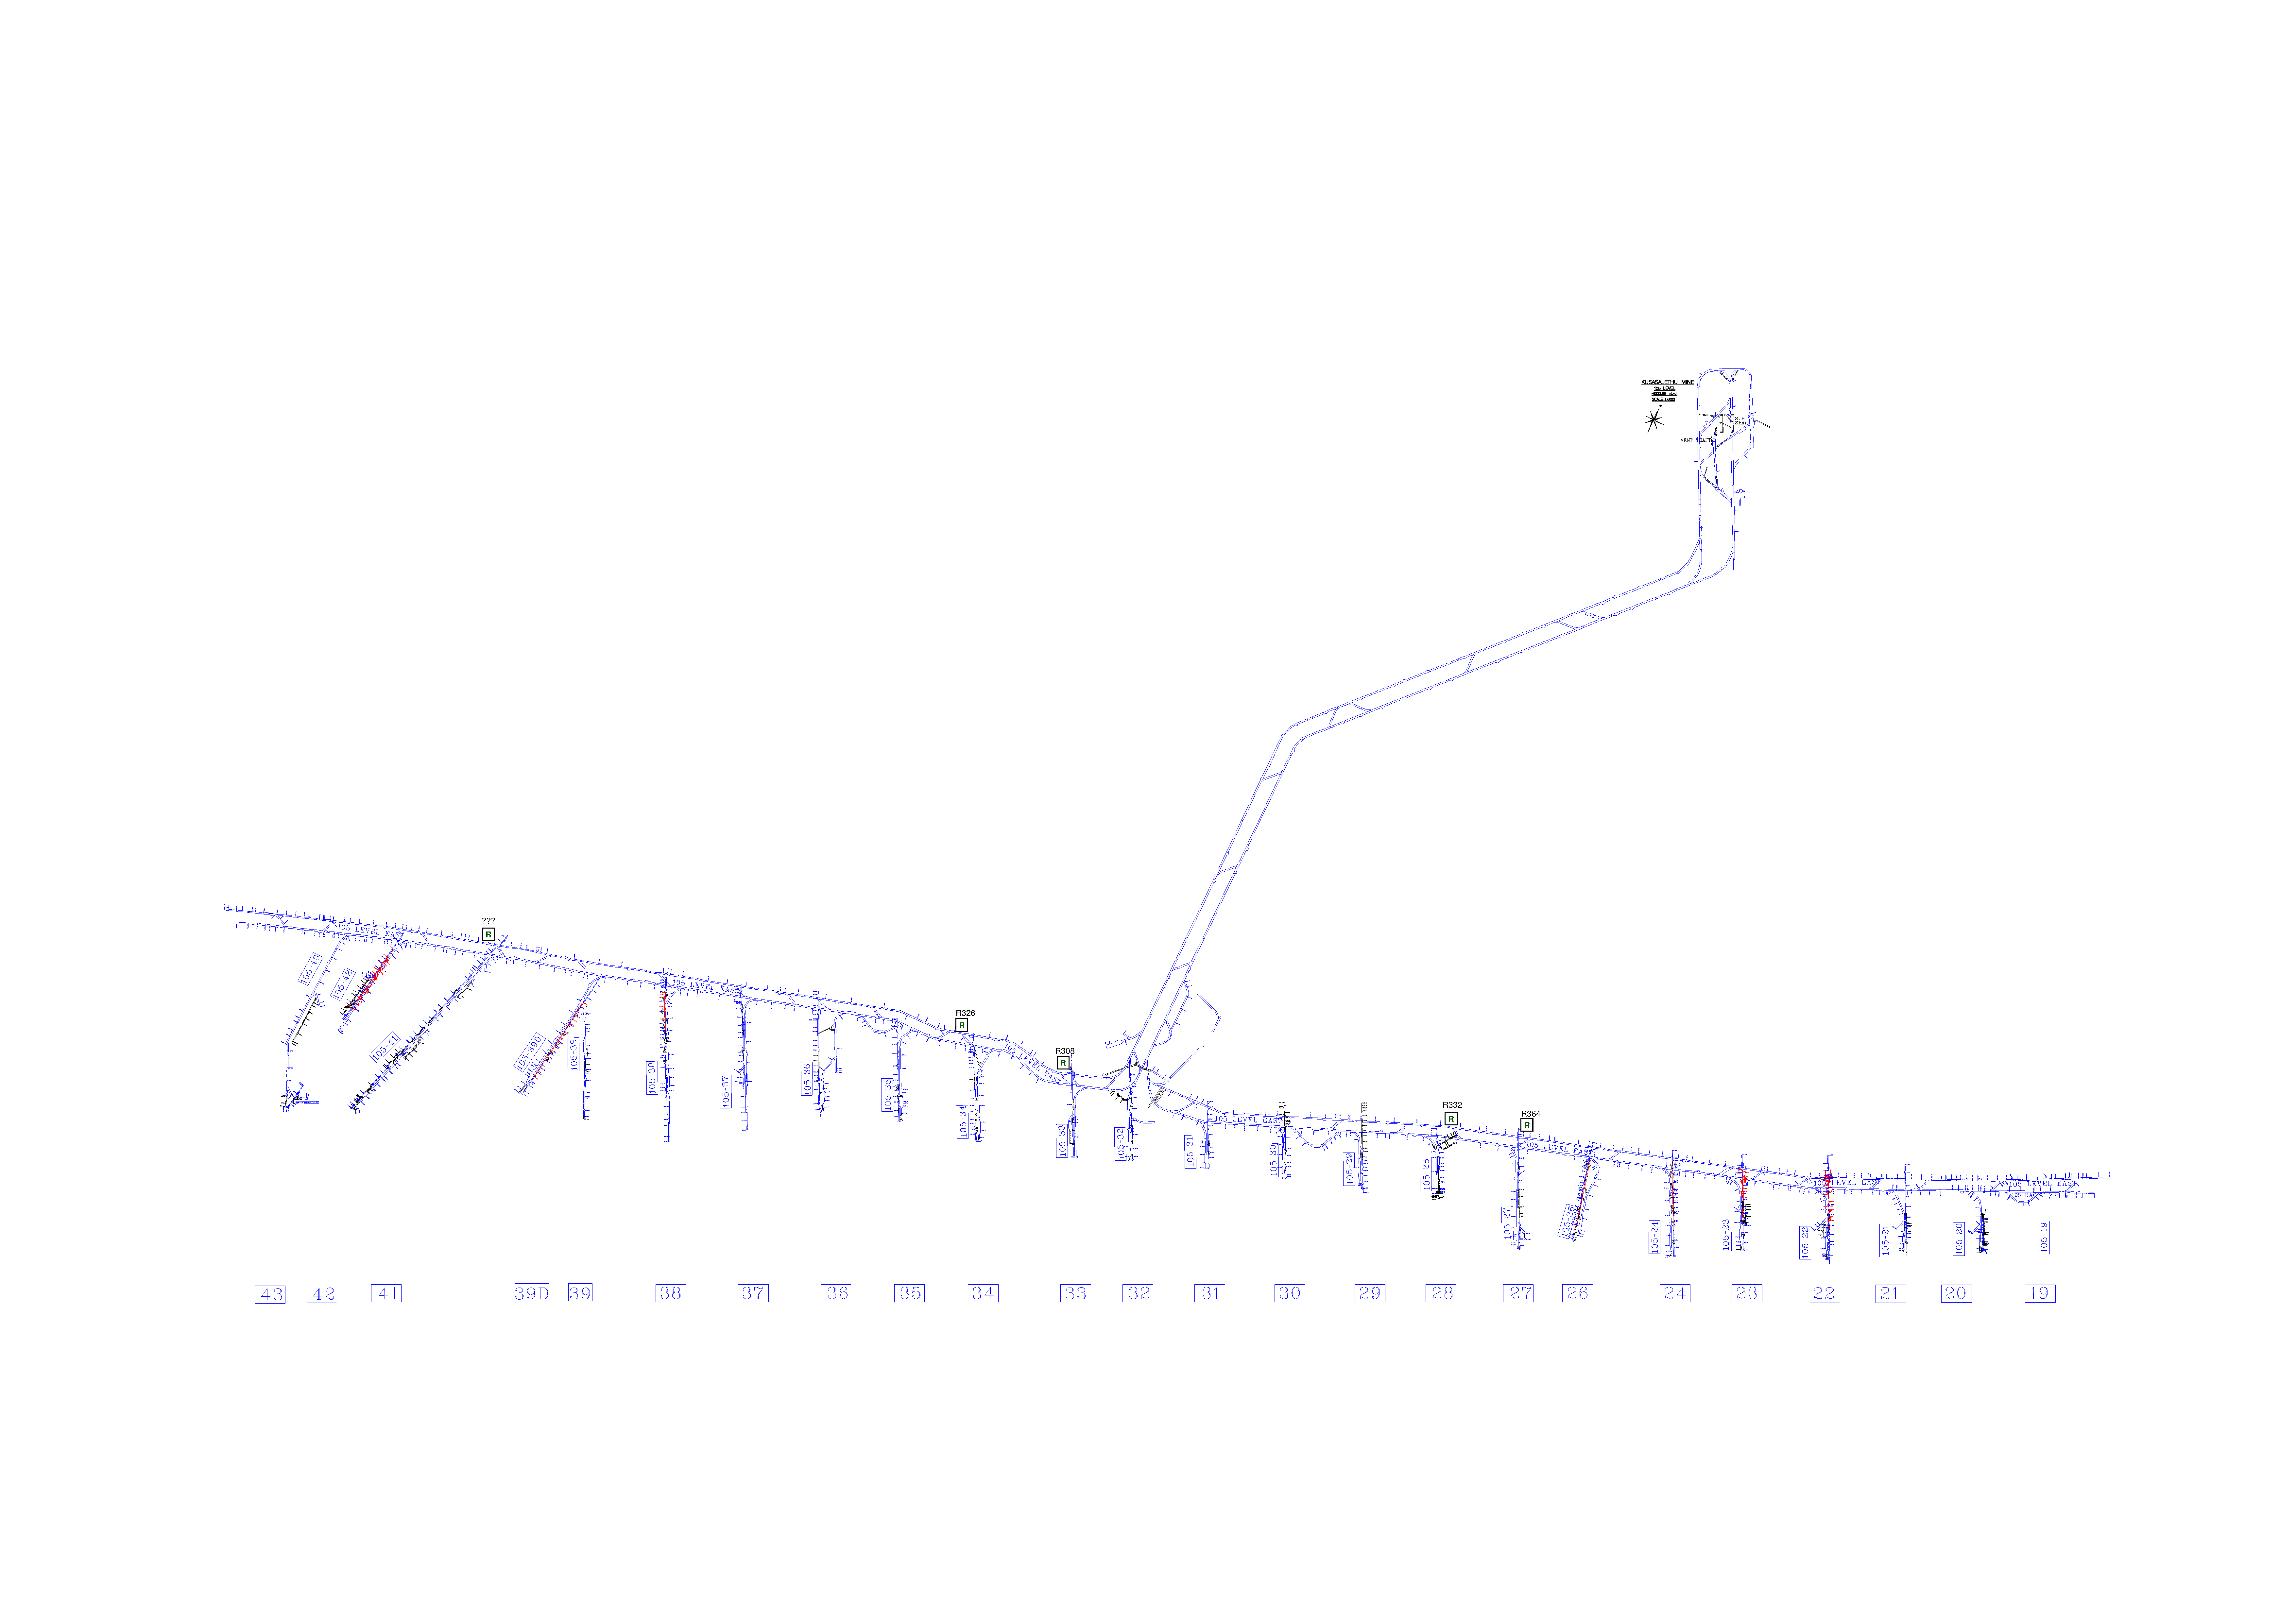
\includegraphics[trim =9cm 12cm 9cm 15cm,angle=90, height=0.85\textheight]{Graphs/4/LevelLayout/105L.pdf}}
	\caption{Underground mining level layout}
	\label{fig: KUS Underground level layout}
\end{figure}
\end{appendices}
